\documentclass{../../slides-style}

\slidetitle{Лекция 5: Проектирование пользовательских интерфейсов}{26.03.2024}

\begin{document}

    \begin{frame}[plain]
        \titlepage
    \end{frame}

    \section{Понятие UX}

    \begin{frame}
        \frametitle{Современное ПО}
        \begin{columns}
            \begin{column}{0.5\textwidth}
                \begin{itemize}
                    \item Высокая доступность
                    \item Высокая конкурентность
                    \item Важна не только функциональность
                    \begin{itemize}
                        \item Сервис
                        \item Look and feel
                    \end{itemize}
                \end{itemize}
            \end{column}
            \begin{column}{0.5\textwidth}
                \begin{center}
                    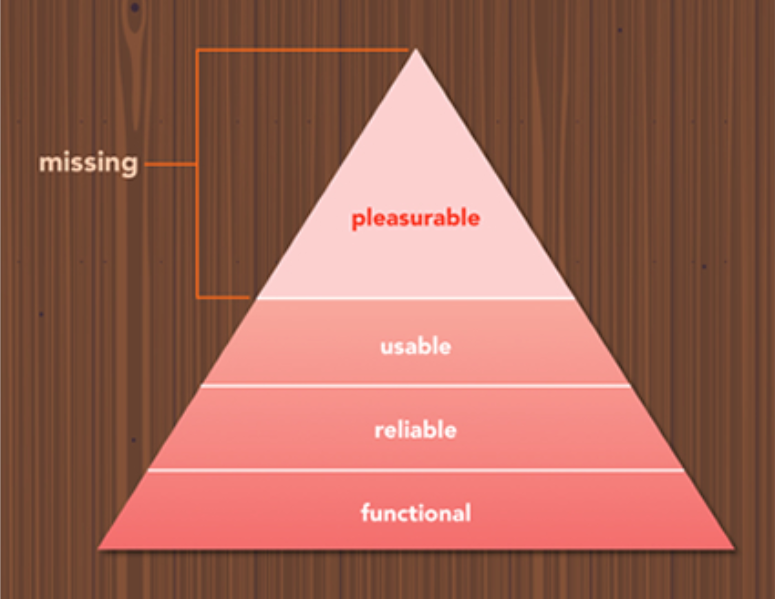
\includegraphics[width=0.8\textwidth]{uxPyramid.png}
                \end{center}
            \end{column}
        \end{columns}
    \end{frame}

    \begin{frame}
        \frametitle{User eXperience}
        \begin{columns}
            \begin{column}{0.5\textwidth}
                \begin{itemize}
                    \item Восприятие продукта, эмоции, ощущения, физические и психологические реакции
                    \item До, во время и после использования продукта
                \end{itemize}
            \end{column}
            \begin{column}{0.5\textwidth}
                \begin{center}
                    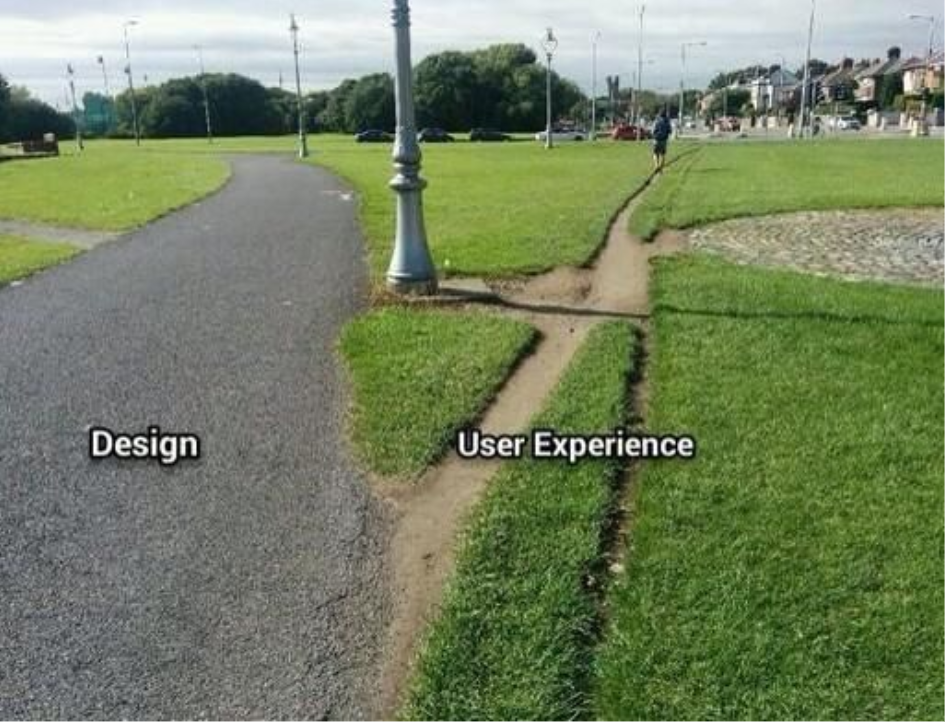
\includegraphics[width=0.9\textwidth]{uxWay.png}
                \end{center}
            \end{column}
        \end{columns}
    \end{frame}

    \begin{frame}
        \begin{center}
            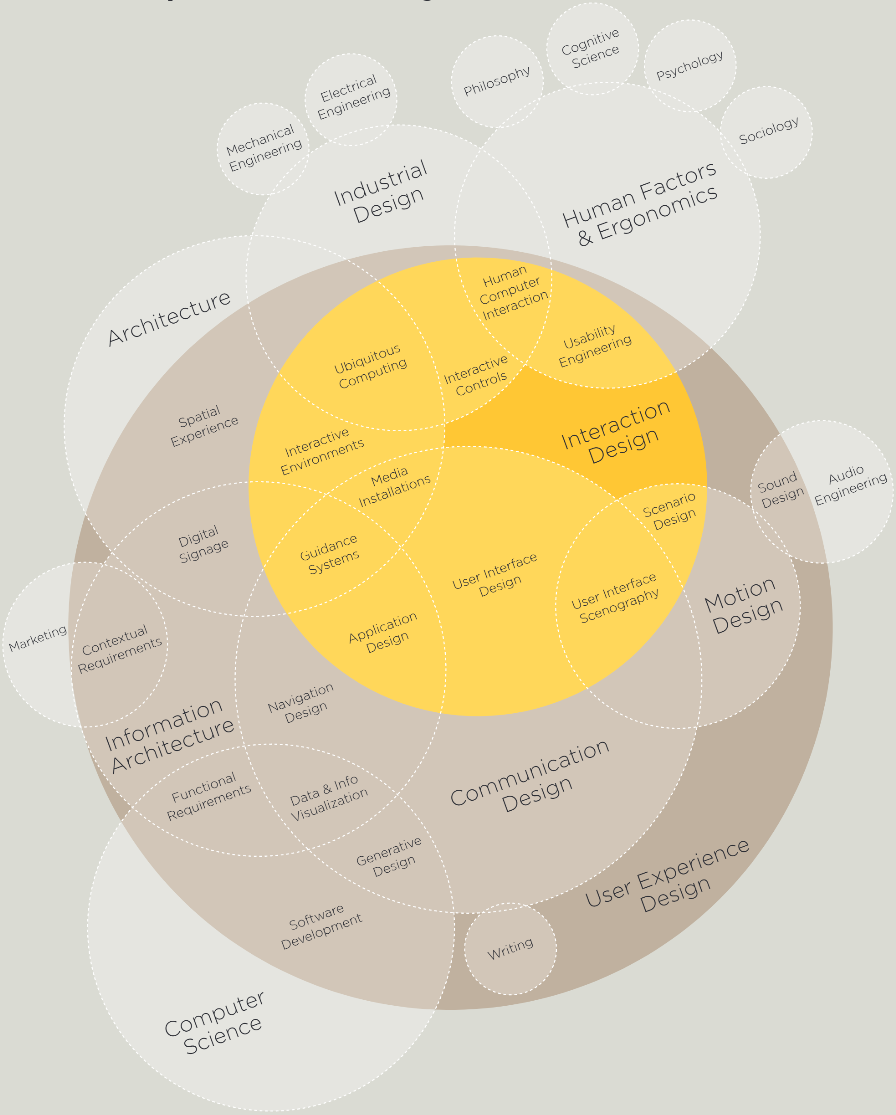
\includegraphics[width=0.5\textwidth]{uxDesign.png}
            \attribution{\url{https://github.com/envisprecisely/disciplines-of-ux}}
        \end{center}
    \end{frame}

    \begin{frame}
        \frametitle{Слои UX}
        \begin{center}
            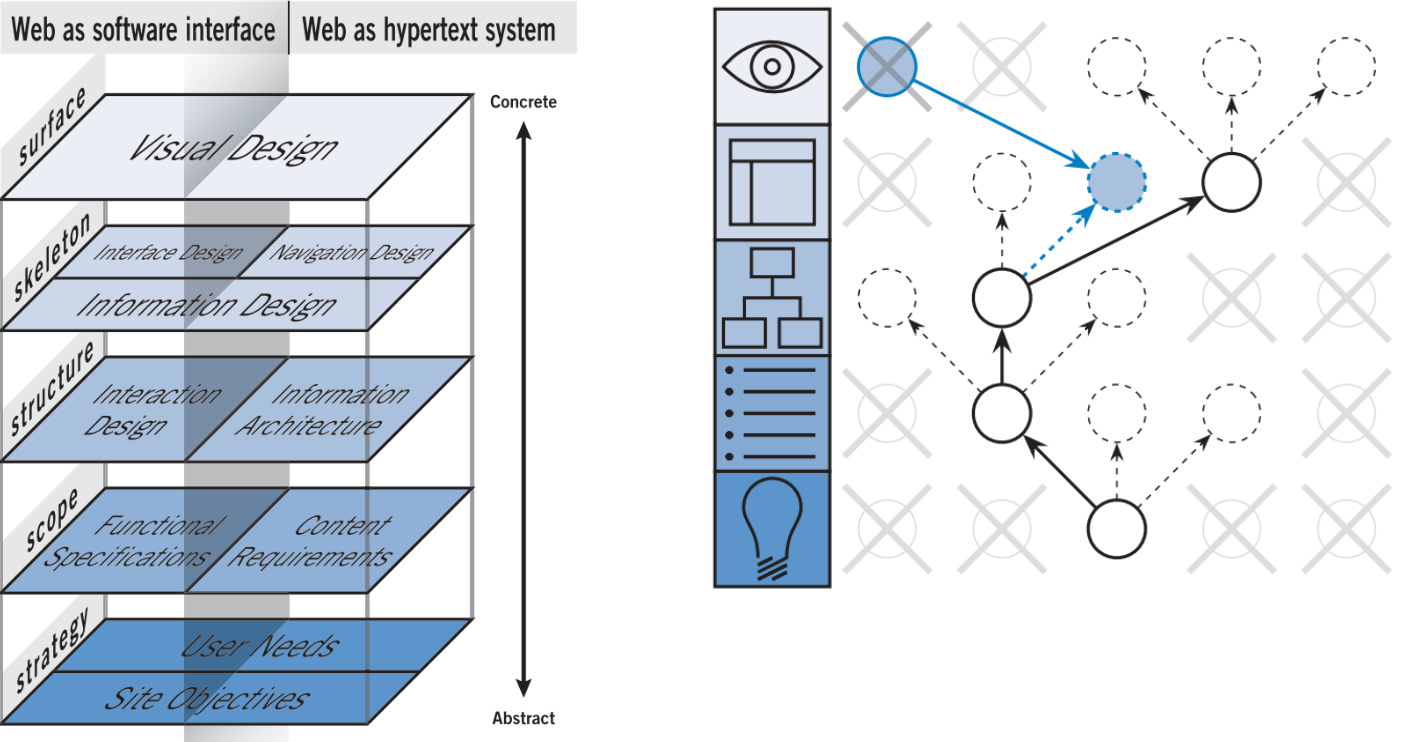
\includegraphics[width=0.9\textwidth]{uxLayers.png}
        \end{center}
    \end{frame}

    \begin{frame}
        \begin{center}
            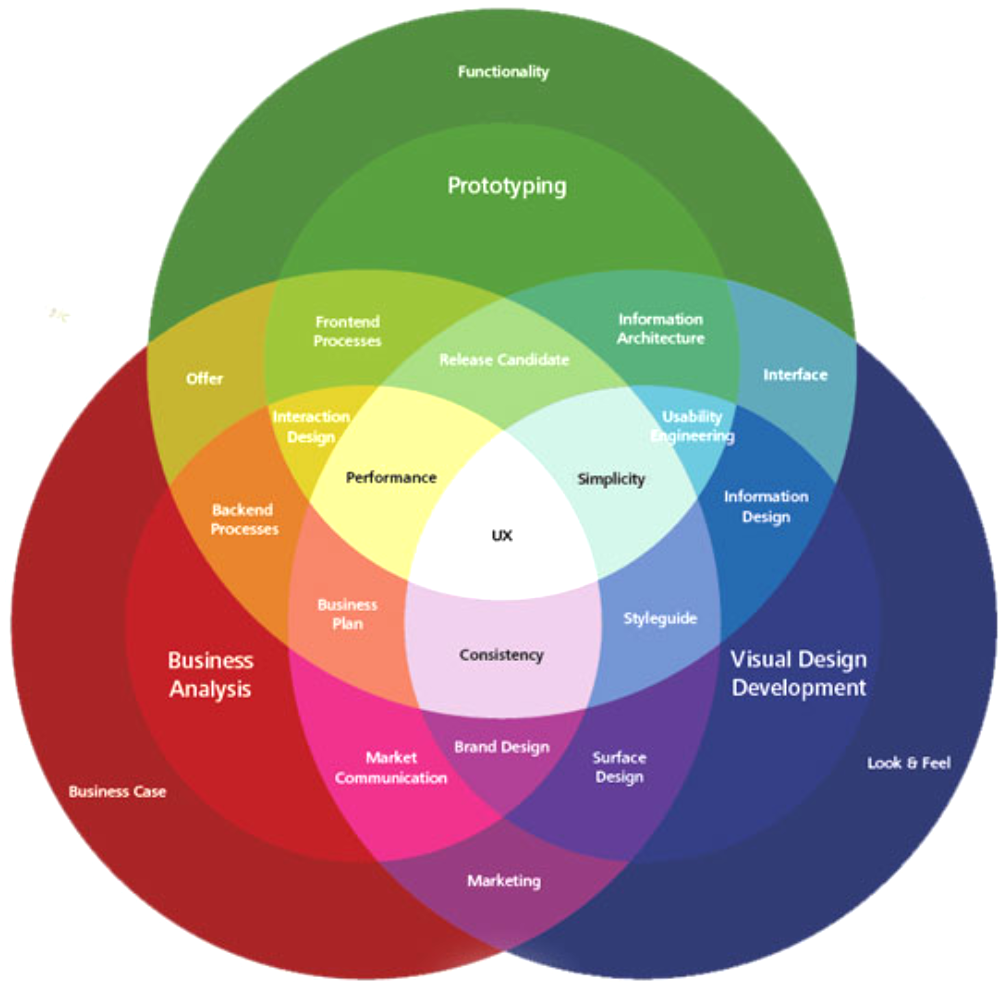
\includegraphics[width=0.7\textwidth]{uxDesignPractices.png}
        \end{center}
    \end{frame}

    \section{Стадии проектирования}

    \begin{frame}
        \frametitle{Стадии проектирования}
        \begin{enumerate}
            \item Предварительные исследования
            \item Стратегия
            \item Информационная структура
            \item Прототипирование
            \item Исследования продукта
        \end{enumerate}
    \end{frame}

    \begin{frame}
        \frametitle{Предварительные исследования}
        \begin{itemize}
            \item Как продукт вписывается в контекст жизни пользователя? 
            \item Каковы основные цели людей в работе с продуктом? 
            \item Какие базовые задачи позволяют достигать целей? 
            \item Какой опыт люди находят привлекательным? Как он соотносится с продуктом?
            \item Какие проблемы встречаются у людей?
        \end{itemize}
    \end{frame}

    \begin{frame}
        \frametitle{Стратегия}
        \begin{itemize}
            \item Что за продукт разрабатывается?
            \item Для кого?
            \item Что он в итоге будет собой представлять?
            \item Какие бизнес-цели?
        \end{itemize}
    \end{frame}

    \section{User-centered design}

    \begin{frame}
        \frametitle{User-centered design}
        \begin{columns}
            \begin{column}{0.5\textwidth}
                \begin{itemize}
                    \item В основе всего потребности пользователей
                \end{itemize}
                Для \textcolor{green}{(целевых пользователей)}, которым нужно \textcolor{green}{(потребность)}, \textcolor{green}{(Название продукта)} --- это \textcolor{green}{(рыночная категория)}, который \textcolor{green}{(одно ключевое преимущество)}.

                \vspace{5mm}

                В отличие от \textcolor{green}{(конкуренты)}, \textcolor{green}{(Название продукта)} \textcolor{green}{(уникальное отличие)}.
            \end{column}
            \begin{column}{0.5\textwidth}
                \begin{center}
                    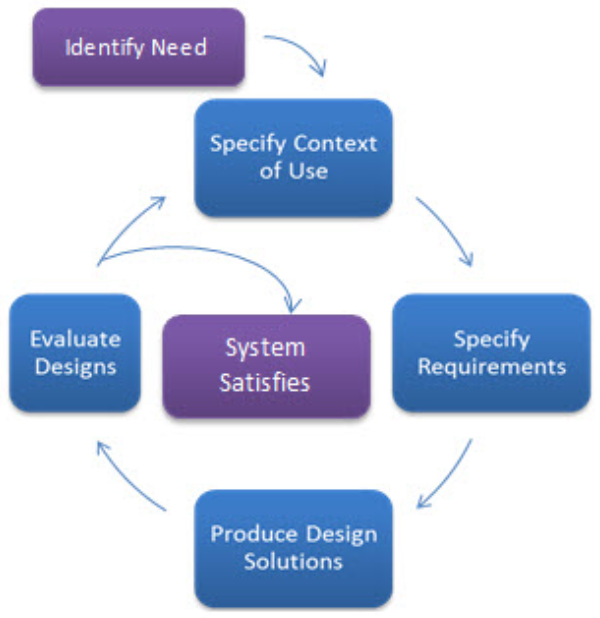
\includegraphics[width=0.8\textwidth]{userCenteredDesignLoop.png}
                \end{center}
            \end{column}
        \end{columns}
    \end{frame}

    \begin{frame}
        \frametitle{Персонажи}
        \begin{itemize}
            \item Модели основных типов пользователей
            \begin{itemize}
                \item Мотивация
                \item Цели
                \item Поведенческие шаблоны
            \end{itemize}
            \item 2-4 групп пользователей
            \begin{itemize}
                \item Какие наиболее важные?
            \end{itemize}
            \item Помогают решать проблемы
            \begin{itemize}
                \item Проектирование под себя
                \item Пластилиновый пользователь
                \item Расчёт на исключительные ситуации
            \end{itemize}
        \end{itemize}
    \end{frame}

    \begin{frame}
        \begin{center}
            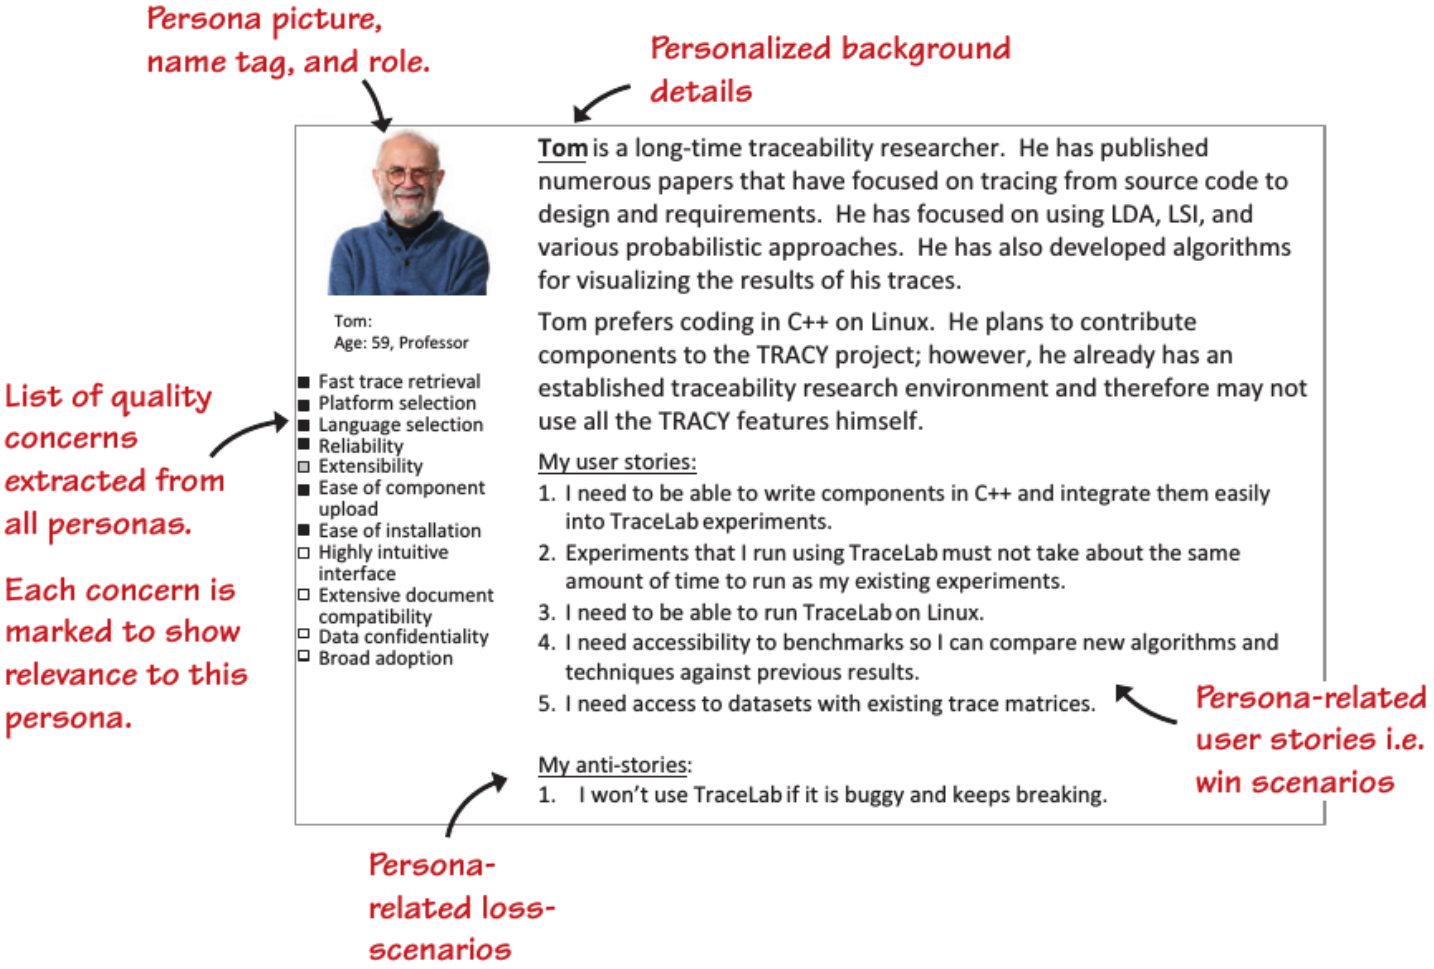
\includegraphics[width=\textwidth]{tom.png}
        \end{center}
    \end{frame}

    \begin{frame}
        \begin{center}
            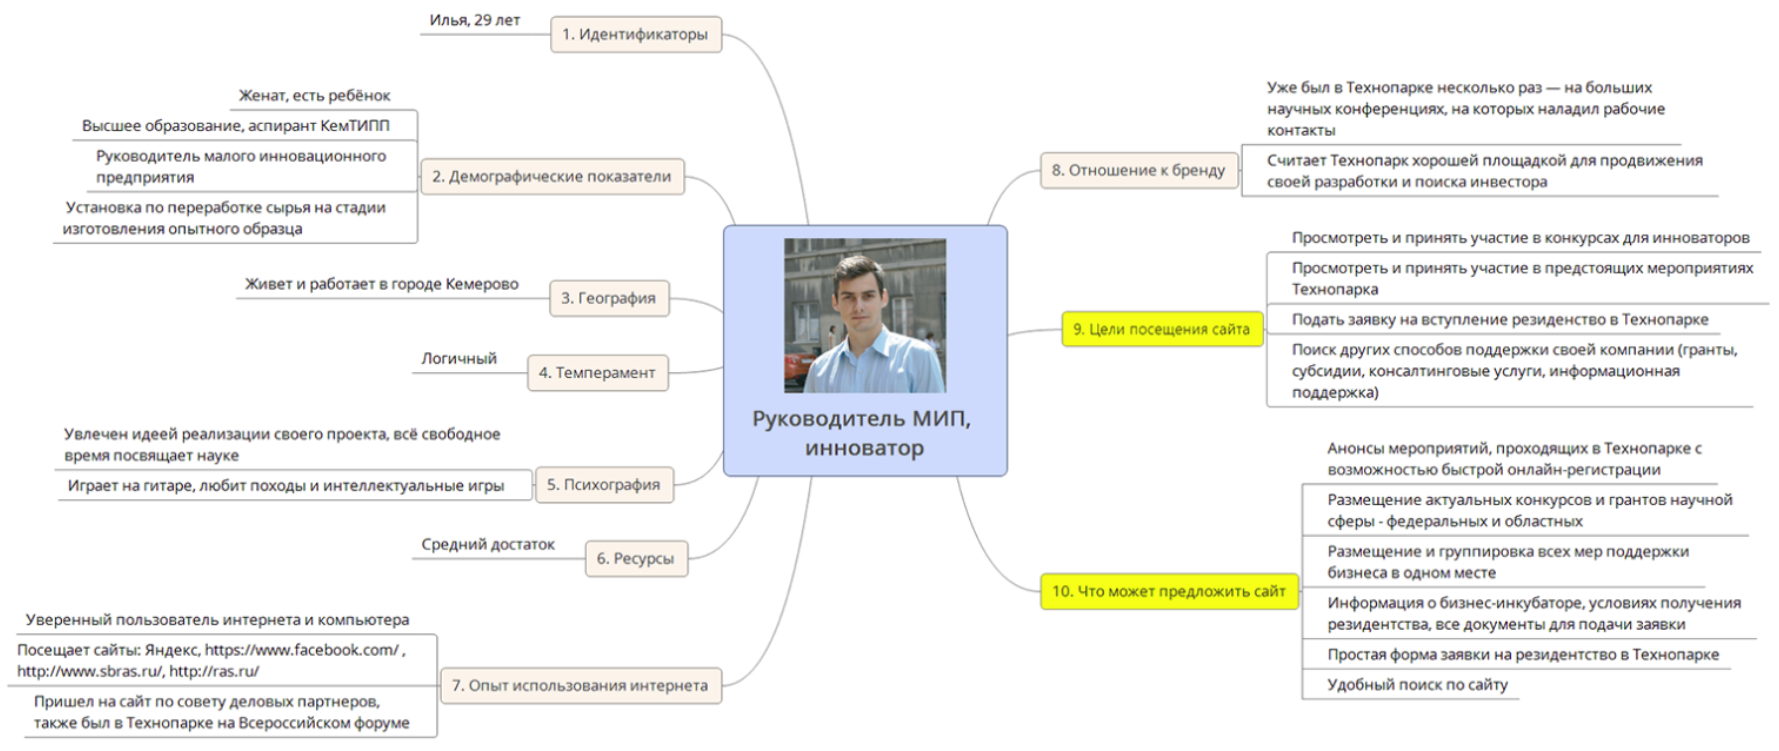
\includegraphics[width=\textwidth]{ilya.png}
        \end{center}
    \end{frame}

    \begin{frame}
        \frametitle{Время на создание персонажей}
        \begin{center}
            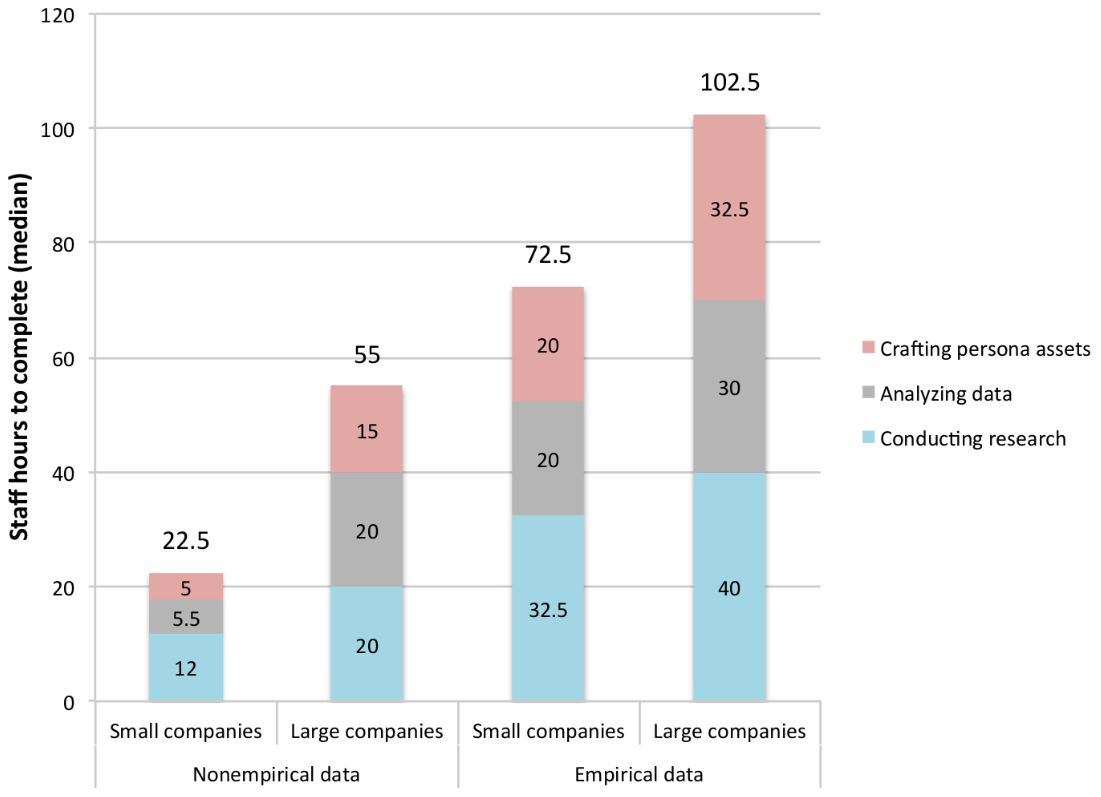
\includegraphics[width=0.8\textwidth]{createCharactersTime.png}
        \end{center}
    \end{frame}

    \begin{frame}
        \begin{center}
            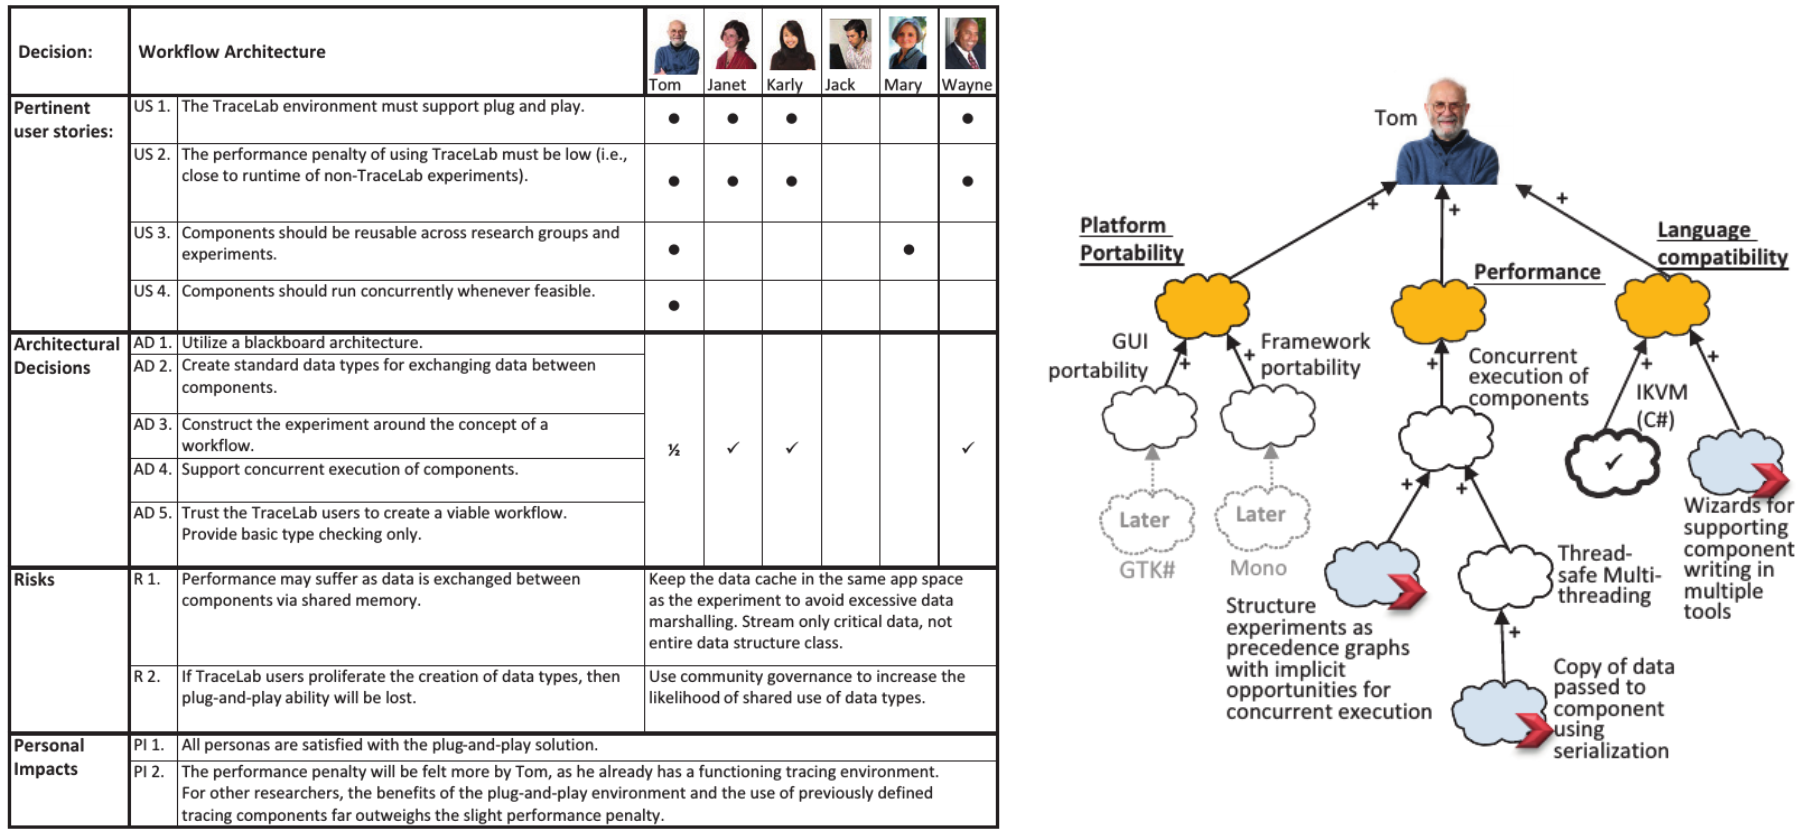
\includegraphics[width=\textwidth]{decisions.png}
        \end{center}
    \end{frame}

    \begin{frame}
        \frametitle{Сценарии}
        \begin{itemize}
            \item Повествование об использовании продукта
            \item Описывают идеальное (для пользователя) взаимодействие
            \item Варианты сценариев
            \begin{itemize}
                \item Контекстные сценарии
                \item Сценарии ключевого пути
                \item Проверочные сценарии
            \end{itemize}
        \end{itemize}
    \end{frame}

    \section{Activity-centered design}

    \begin{frame}
        \frametitle{Activity-centred design}
        \begin{itemize}
            \item Ориентация на действия, которые совершаются для решения задачи
            \item Пользователей может быть много
            \item Пользователи могут не знать, что хотят
            \item Люди хорошо адаптируются под технологии
        \end{itemize}
    \end{frame}

    \section{Data-driven design}

    \begin{frame}
        \frametitle{Data-driven design}
        \begin{itemize}
            \item В основе --- данные
            \begin{itemize}
                \item Публичная или инсайдерская информация о конкурентах
                \item Маркетинговые отчёты и статьи
                \item Данные нашего приложения
            \end{itemize}
        \end{itemize}
        \begin{center}
            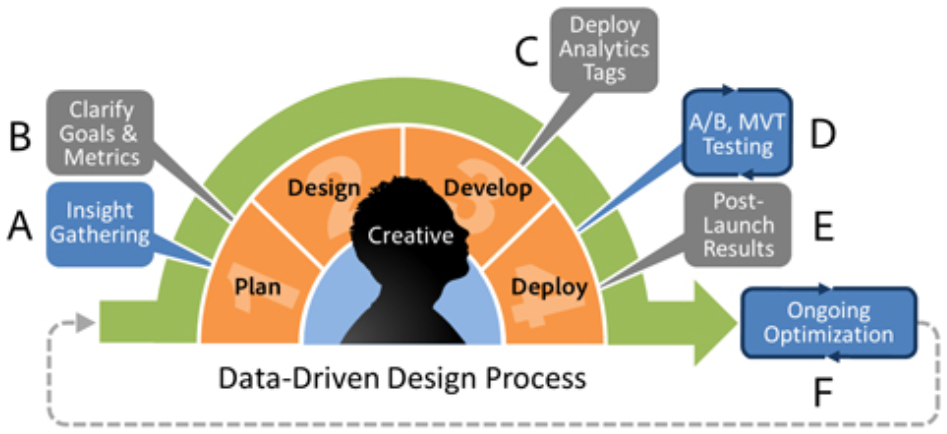
\includegraphics[width=0.6\textwidth]{dataDrivenDesign.png}
        \end{center}
    \end{frame}

    \begin{frame}
        \frametitle{Информационная структура}
        \begin{columns}
            \begin{column}{0.4\textwidth}
                \begin{itemize}
                    \item Архитектура
                    \begin{itemize}
                        \item системы
                        \item взаимодействия с ней
                    \end{itemize}
                    \item Типы
                    \begin{itemize}
                        \item Категории
                        \item Задачи
                        \item Поиск
                        \item Время
                        \item Люди
                    \end{itemize}
                \end{itemize}
            \end{column}
            \begin{column}{0.6\textwidth}
                \begin{center}
                    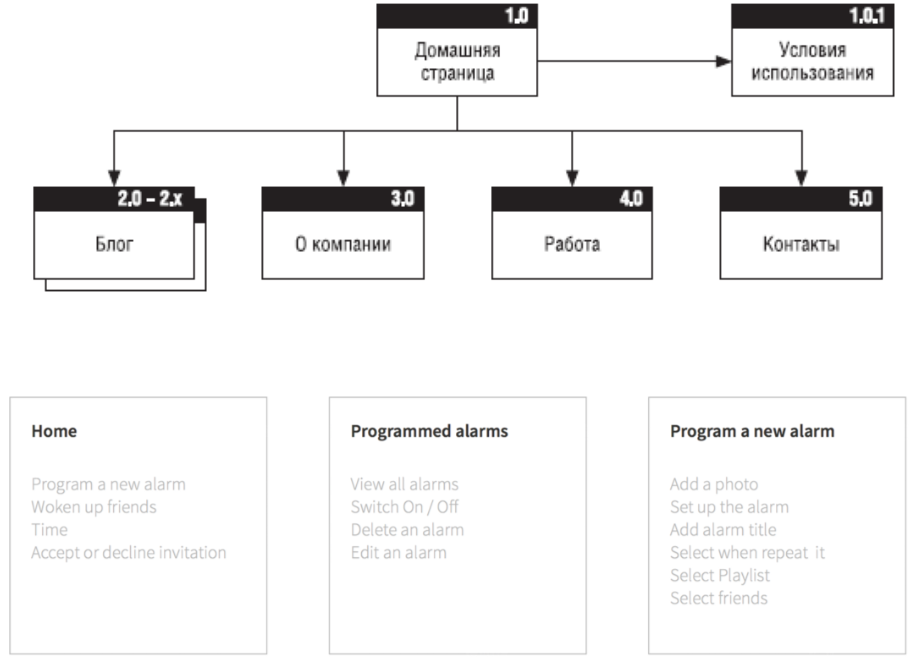
\includegraphics[width=\textwidth]{informationStructure.png}
                \end{center}
            \end{column}
        \end{columns}
    \end{frame}

    \begin{frame}
        \frametitle{Табличное представление (1)}
        \begin{center}
            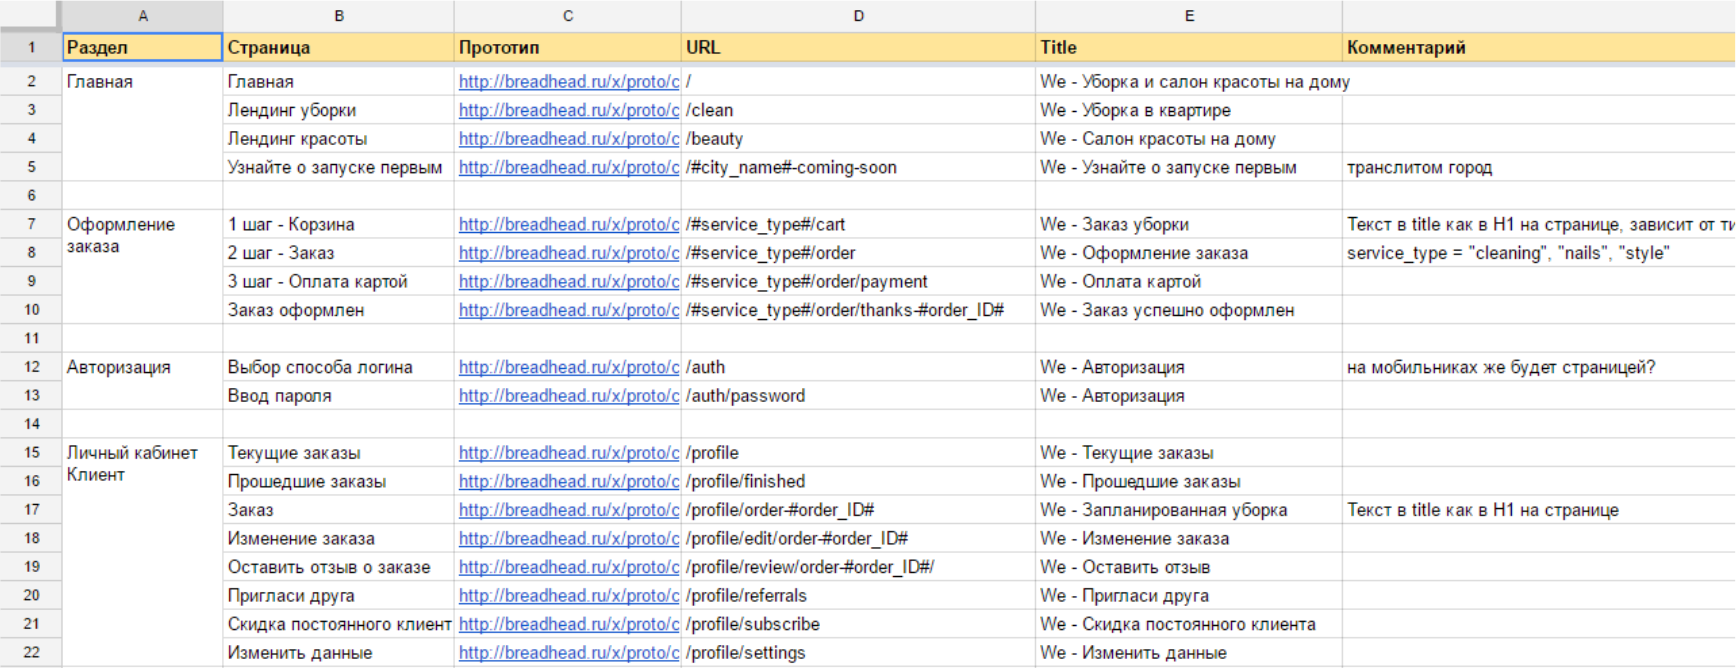
\includegraphics[width=\textwidth]{tableView1.png}
        \end{center}
    \end{frame}

    \begin{frame}
        \frametitle{Табличное представление (2)}
        \begin{center}
            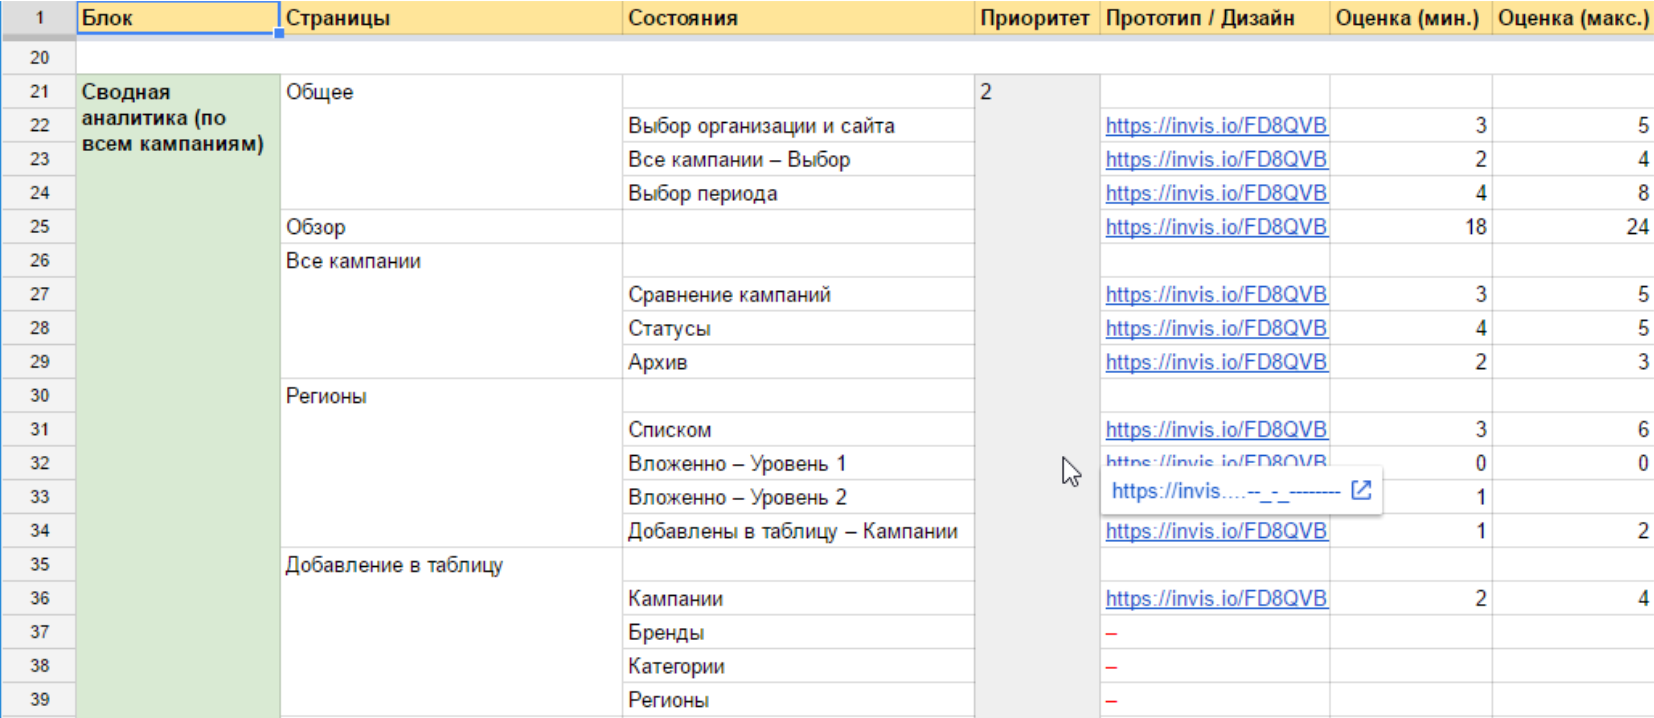
\includegraphics[width=\textwidth]{tableView2.png}
        \end{center}
    \end{frame}

    \begin{frame}
        \frametitle{Customer Journey Maps}
        \begin{center}
            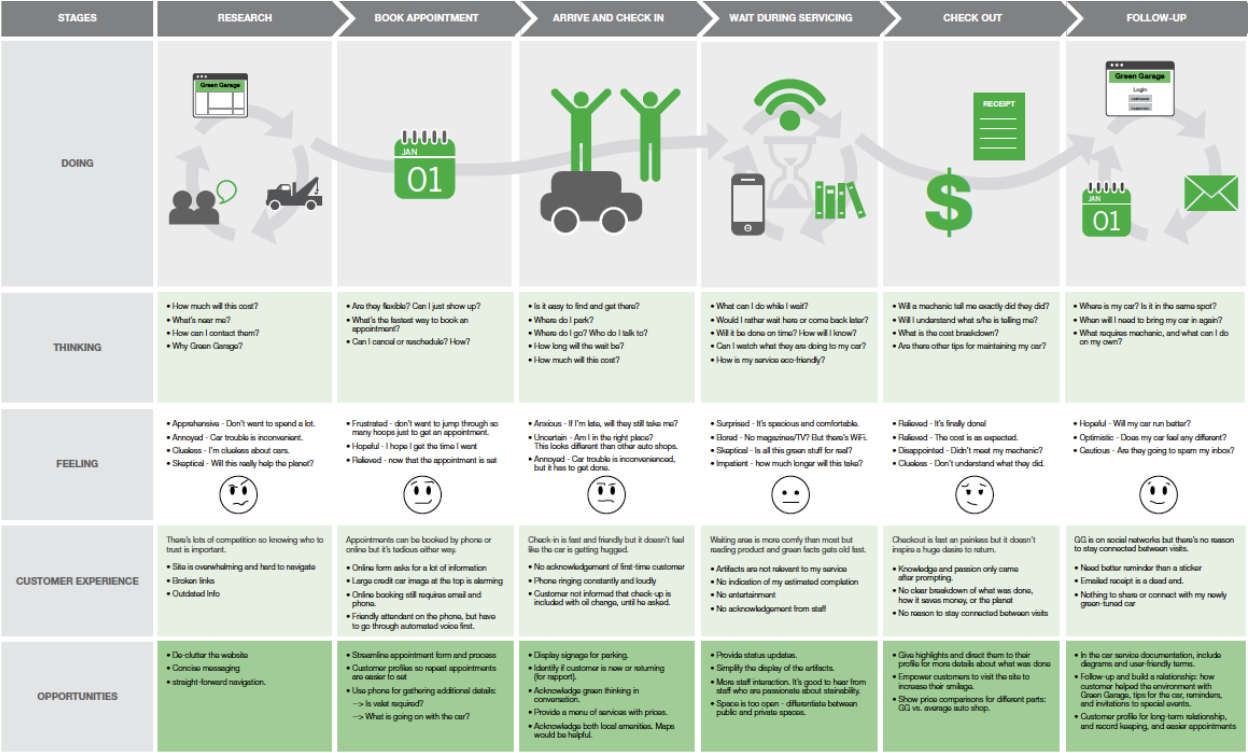
\includegraphics[width=\textwidth]{customerJourneyMaps.png}
        \end{center}
    \end{frame}

    \section{Прототипирование}

    \begin{frame}
        \frametitle{Прототипирование}
        \begin{itemize}
            \item Storytelling
            \item Storyboarding
            \item Бумажные прототипы
            \item Bodystorming
            \item Wireframe (макет)
            \item Дизайн-макет (цифровой mockup)
            \item Интерактивный прототип
            \item Прототипирование кодом
        \end{itemize}
    \end{frame}

    \begin{frame}
        \frametitle{Storyboarding (раскадровки)}
        \begin{itemize}
            \item Кто ваш персонаж?
            \item Какую потребность удовлетворяет система?
            \item Какая задача должна быть выполнена?
            \item Что приводит пользователя к использованию вашей системы?
            \item В каких условиях оно выполняется?
            \item Какова последовательность действий?
            \item Какую потребность удовлетворяет приложение?
            \item Какие у пользователей есть возможности?
        \end{itemize}
    \end{frame}

    \begin{frame}
        \frametitle{Пример раскадровки}
        \begin{center}
            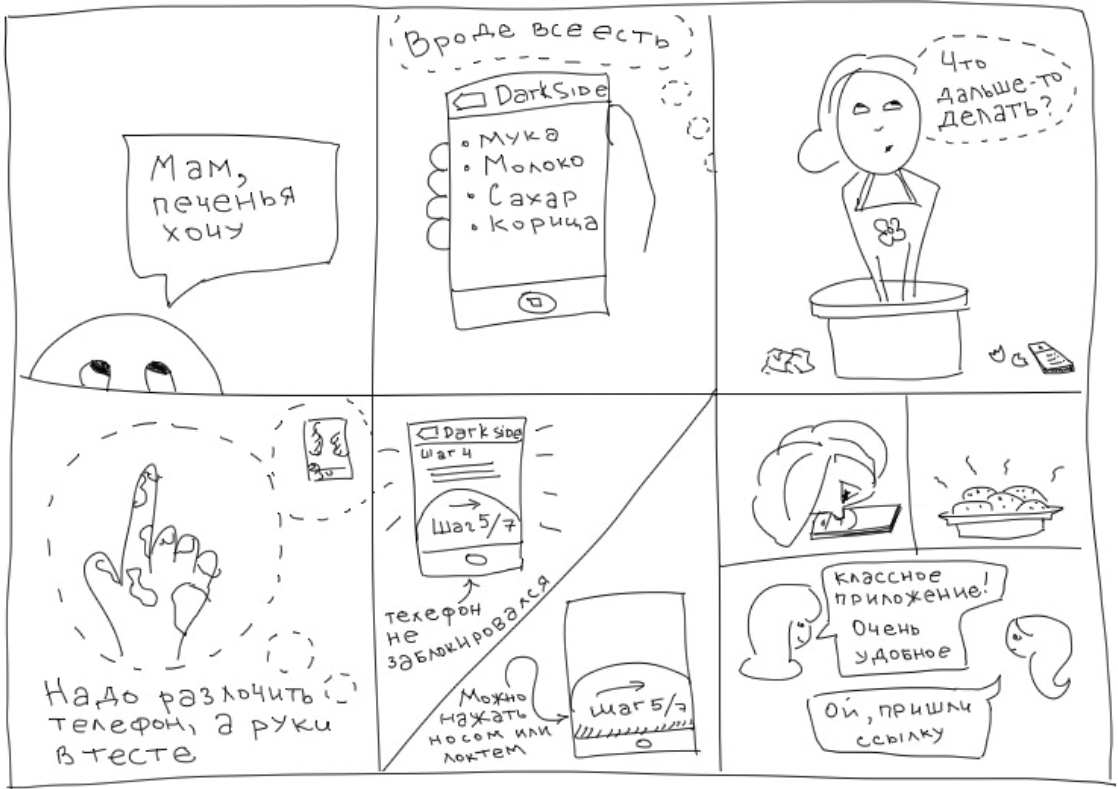
\includegraphics[width=0.8\textwidth]{storyboardingExample.png}
        \end{center}
    \end{frame}

    \begin{frame}
        \frametitle{Бумажные прототипы}
        \begin{columns}
            \begin{column}{0.4\textwidth}
                \begin{itemize}
                    \item Быстро
                    \item Дёшево
                    \item Сердито
                \end{itemize}
                \href{https://www.youtube.com/watch?v=V8LNDqMIapY}{Видео}
            \end{column}
            \begin{column}{0.6\textwidth}
                \begin{center}
                    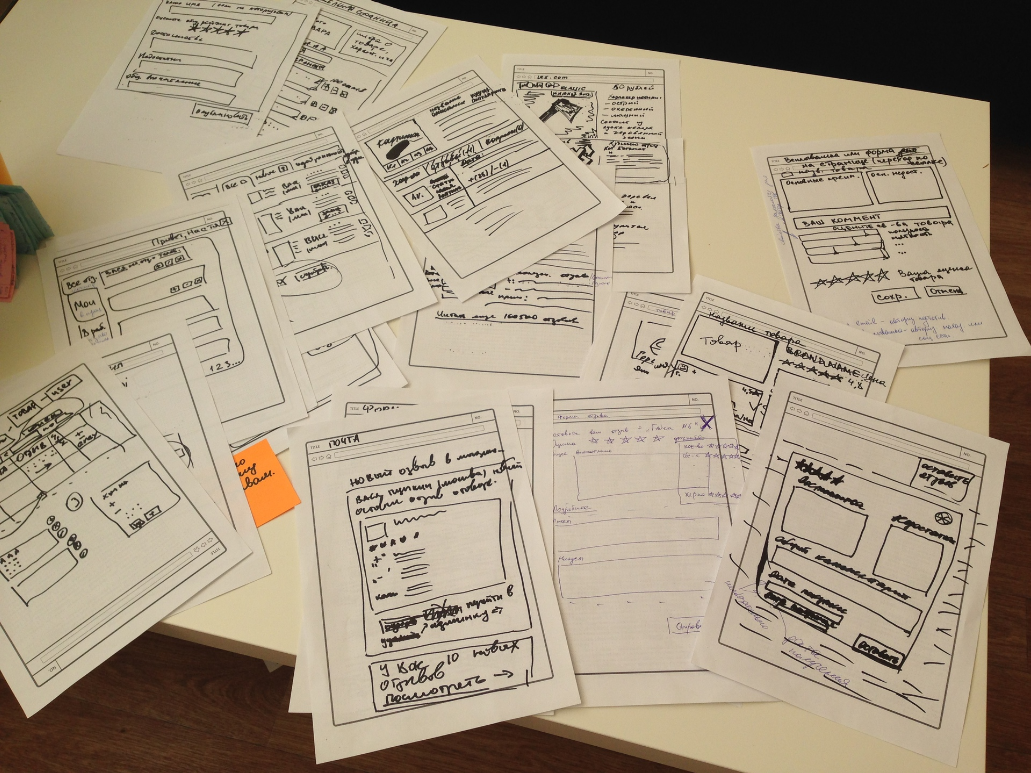
\includegraphics[width=0.8\textwidth]{paperPrototyping.png}
                \end{center}
            \end{column}
        \end{columns}
    \end{frame}

    \begin{frame}
        \frametitle{Bodystorming}
        \href{https://www.youtube.com/watch?v=AoWAnY2La5k}{Видео}
        \begin{center}
            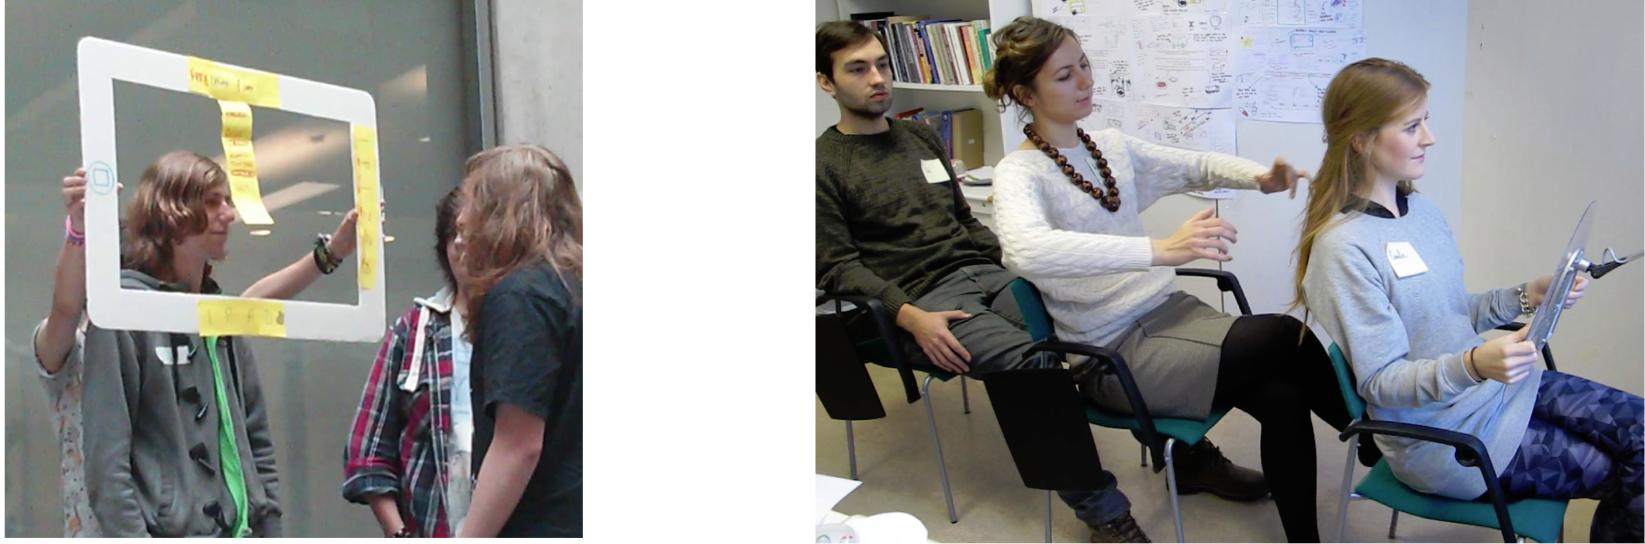
\includegraphics[width=\textwidth]{bodystorming.png}
        \end{center}
    \end{frame}

    \begin{frame}
        \frametitle{Wireframe}
        \begin{columns}
            \begin{column}{0.5\textwidth}
                \begin{itemize}
                    \item Набор схематичных макетов экранов или страниц
                    \item Высокоуровневый внешний вид экранов
                    \begin{itemize}
                        \item Компоновка графических элементов
                    \end{itemize}
                    \item Назначение
                    \begin{itemize}
                        \item ТЗ графическому дизайнеру
                        \item ТЗ программистам
                        \item Наглядный материал для демонстрации
                    \end{itemize}
                \end{itemize}
            \end{column}
            \begin{column}{0.5\textwidth}
                \begin{center}
                    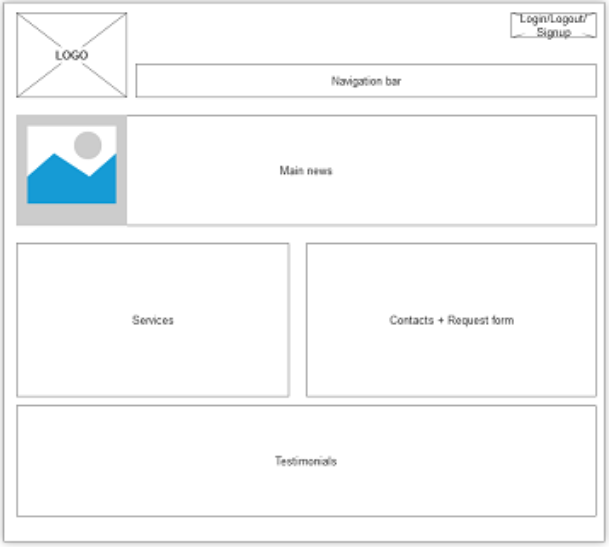
\includegraphics[width=\textwidth]{wireframe.png}
                \end{center}
            \end{column}
        \end{columns}
    \end{frame}

    \begin{frame}
        \frametitle{Пример: сервис для изучения языка}
        \begin{center}
            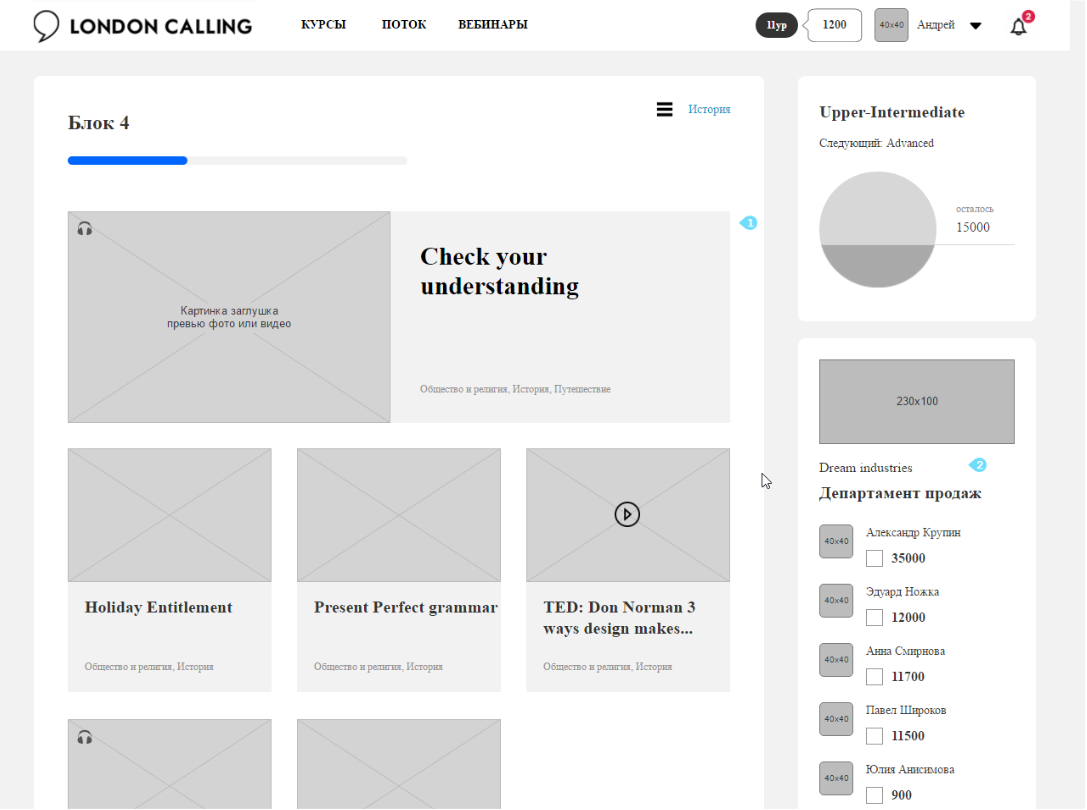
\includegraphics[width=0.8\textwidth]{languageServiceWireframe.png}
        \end{center}
    \end{frame}

    \begin{frame}
        \frametitle{Дизайн-макет}
        \begin{center}
            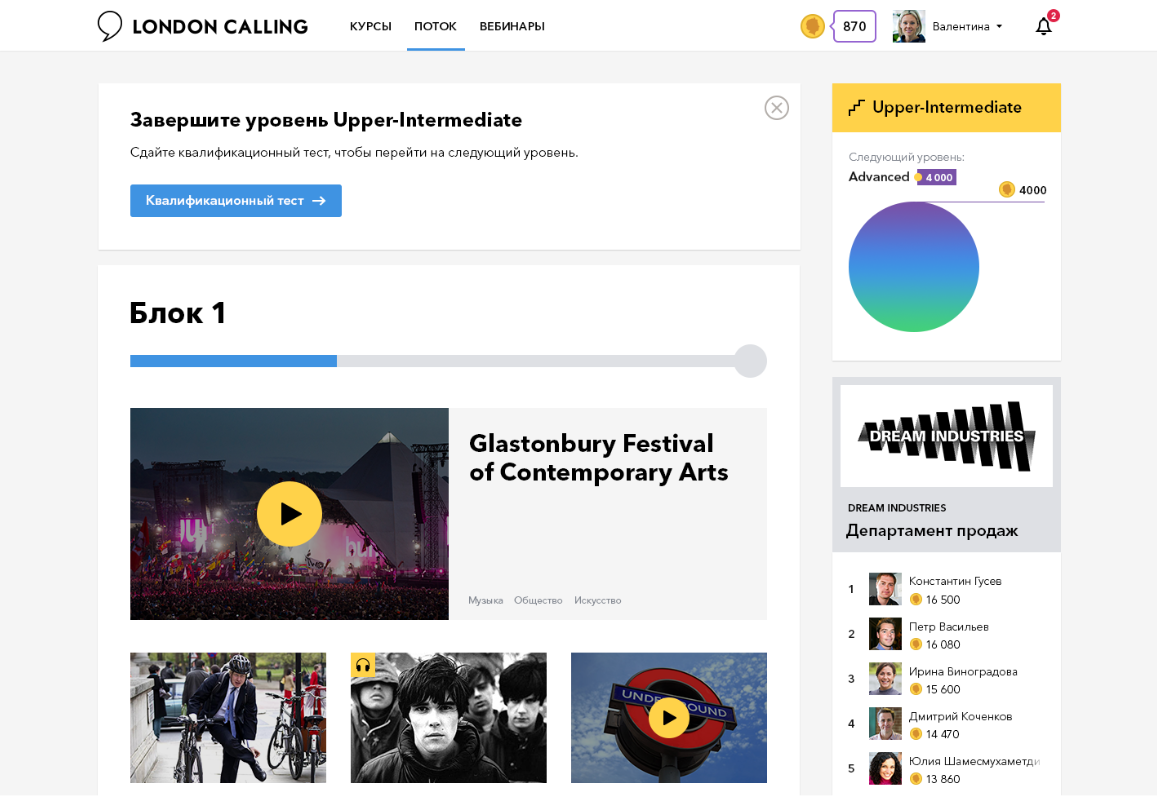
\includegraphics[width=0.8\textwidth]{designLayout.png}
        \end{center}
    \end{frame}

    \begin{frame}
        \begin{center}
            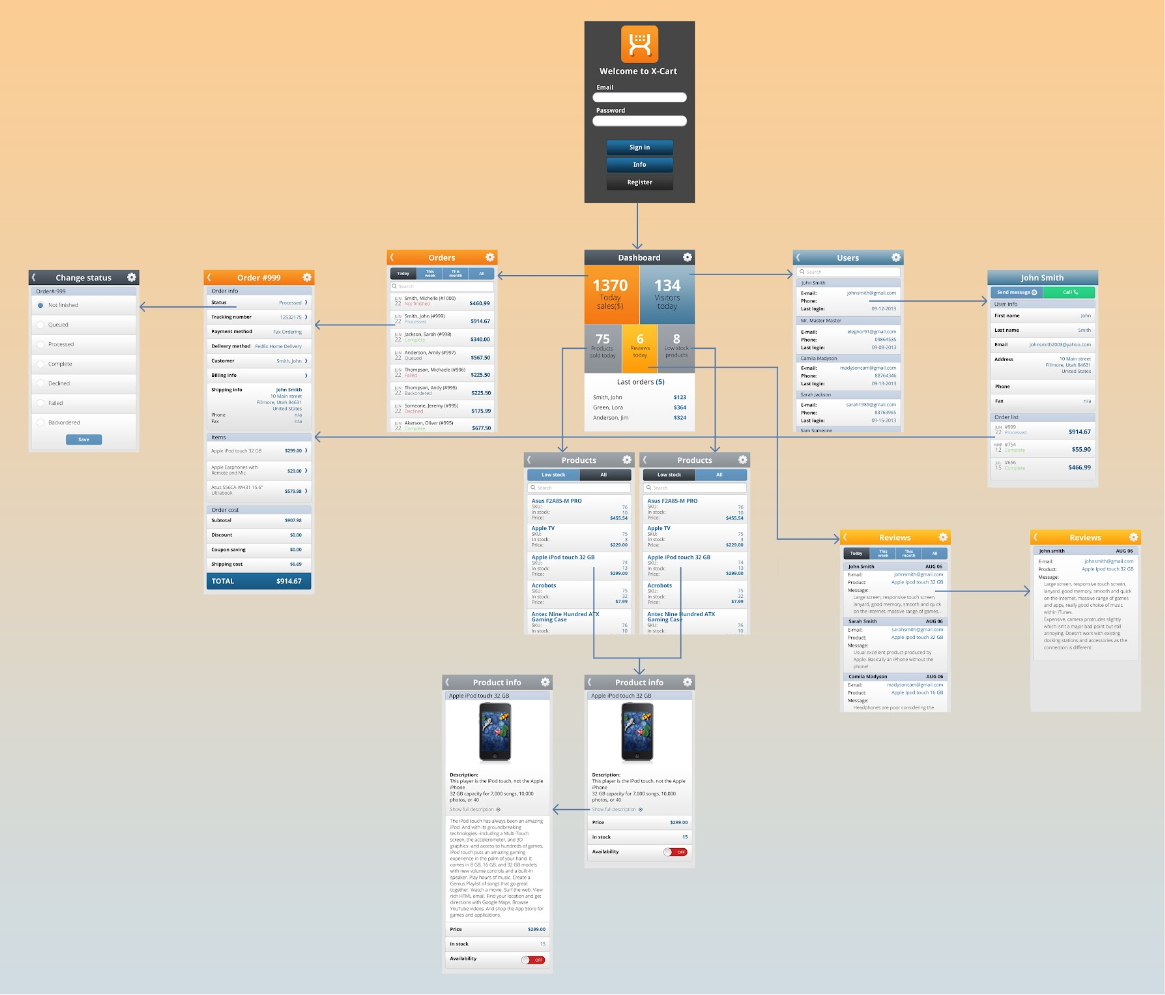
\includegraphics[width=0.8\textwidth]{screenMap.png}
        \end{center}
    \end{frame}

    \begin{frame}
        \frametitle{Интерактивные прототипы}
        \begin{center}
            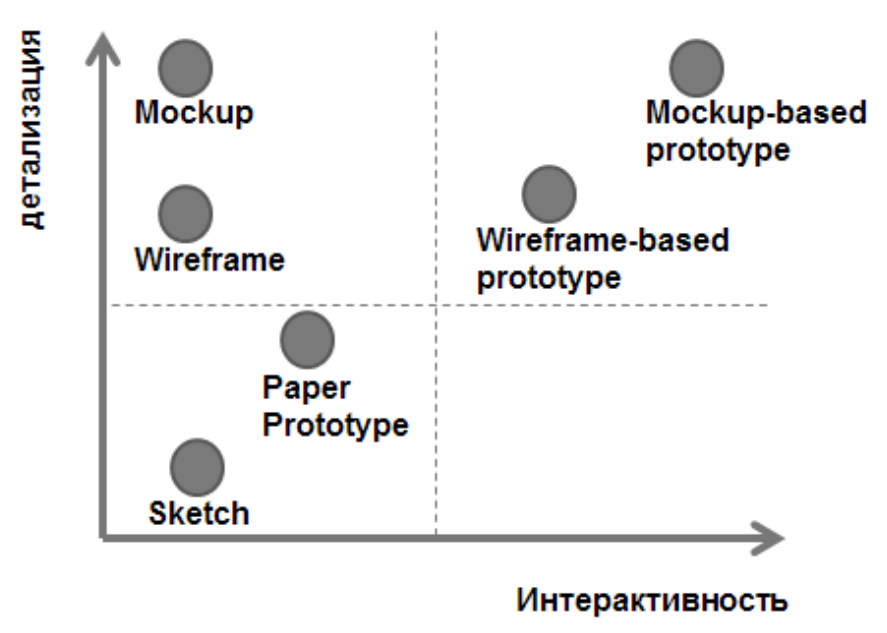
\includegraphics[width=0.7\textwidth]{prototypeClassification.png}
        \end{center}
    \end{frame}

    \begin{frame}
        \frametitle{Немного статистики}
        \begin{center}
            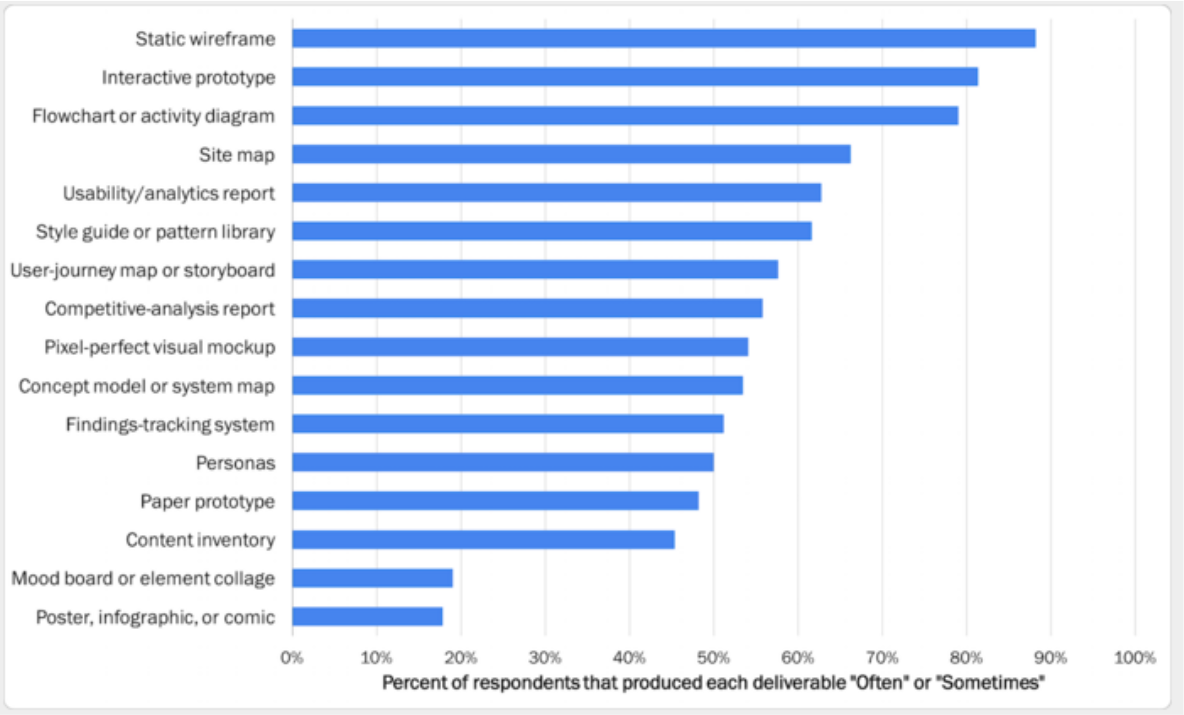
\includegraphics[width=0.8\textwidth]{statistics.png}
        \end{center}
    \end{frame}

    \begin{frame}
        \frametitle{Инструменты проектирования пользовательских интерфейсов}
        \begin{itemize}
            \item Balsamiq
            \begin{itemize}
                \item \url{https://balsamiq.com/products/mockups/}
                \item Кликабельные .pdf-ки
            \end{itemize}
            \item Ninjamock
            \begin{itemize}
                \item \url{https://ninjamock.com/}
                \item Бесплатный
                \item Веб-версия с коллаборацией
            \end{itemize}
            \item Axure
            \begin{itemize}
                \item \url{http://www.axure.com/}
                \item Продвинутый, но платный
            \end{itemize}
            \item UXPin
            \begin{itemize}
                \item \url{https://www.uxpin.com/}
                \item Продвинутый, но платный
                \item Зато браузерный
            \end{itemize}
        \end{itemize}
    \end{frame}

    \begin{frame}
        \frametitle{Ещё инструменты}
        \begin{itemize}
            \item Sketch
            \begin{itemize}
                \item \url{https://www.sketchapp.com/}
                \item Только под Mac
                \item Рисовалка интерфейсов, иконок и прочего
            \end{itemize}
            \item Figma
            \begin{itemize}
                \item \url{https://www.figma.com}
                \item Браузерный, коллаборативный
            \end{itemize}
            \item Invision app
            \begin{itemize}
                \item \url{https://www.invisionapp.com/}
                \item Браузерный, коллаборативный
                \item Кликабельные мокапы из картинок или Sketch-файлов
            \end{itemize}
        \end{itemize}
    \end{frame}

    \section{Исследования продукта}

    \begin{frame}
        \frametitle{Исследования продукта}
        \begin{itemize}
            \item Аудит продукта/прототипа или конкурентов
            \item Экспертная оценка интерфейса
            \item Качественный анализ пользователей (интервью)
            \item Полевое наблюдение (открытое и скрытое)
            \item Анализ данных
            \begin{itemize}
                \item Статистика использования
                \item Выполнение сценариев
                \item Количественный анализ пользователей
            \end{itemize}
            \item A/B-тестирование
            \item Эвристический анализ интерфейса
            \item Usability-исследование
            \begin{itemize}
                \item Фокус-группа
                \item Опросники
                \item Eye tracking
            \end{itemize}
        \end{itemize}
    \end{frame}

    \begin{frame}
        \frametitle{Эвристический анализ Нильсена}
        \begin{enumerate}
            \item Отображение статуса системы
            \item Соответствие между системой и реальным миром
            \item Свобода действий и контроль
            \item Единообразие и стандарты
            \item Профилактика ошибок
            \item Видимость, а не переходы
            \item Гибкость и эффективность использования
            \item Эстетика и минимализм
            \item Помогите пользователям распознавать, диагностировать и исправлять ошибки
            \item Помощь и документация
        \end{enumerate}
    \end{frame}

    \begin{frame}
        \frametitle{Usability-тестирование}
        \begin{columns}
            \begin{column}{0.6\textwidth}
                \begin{itemize}
                    \item не то же, что тестирование GUI
                    \item 8/85
                    \item Шаги
                    \begin{itemize}
                        \item Формирование гипотез
                        \item Определение метрик для тестирования
                        \item Определение персонажей и сценариев
                        \item Подбор респондентов
                        \item Заполнение анкеты
                        \item Вводный инструктаж
                        \item Проведение юзабилити-тестирования
                        \item Опрос респондентов
                        \item Анализ результатов
                        \item Определение требований для проектирования сайта
                    \end{itemize}
                \end{itemize}
            \end{column}
            \begin{column}{0.4\textwidth}
                \begin{center}
                    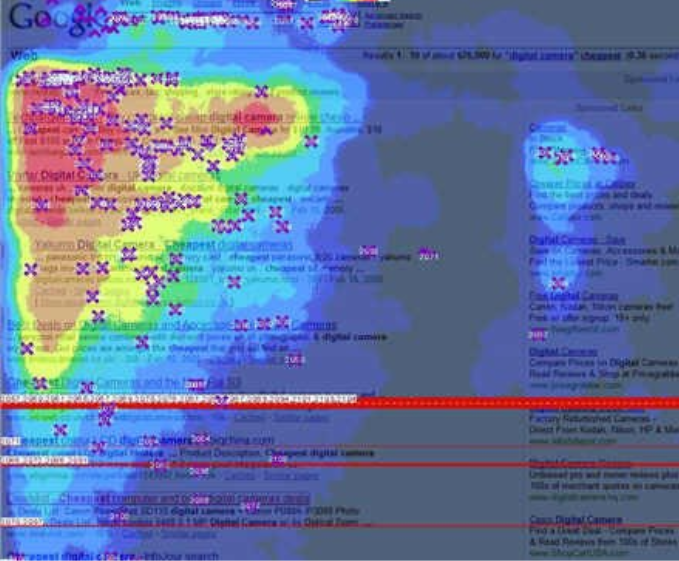
\includegraphics[width=\textwidth]{heatMap.png}
                \end{center}
            \end{column}
        \end{columns}
    \end{frame}

    \begin{frame}
        \begin{center}
            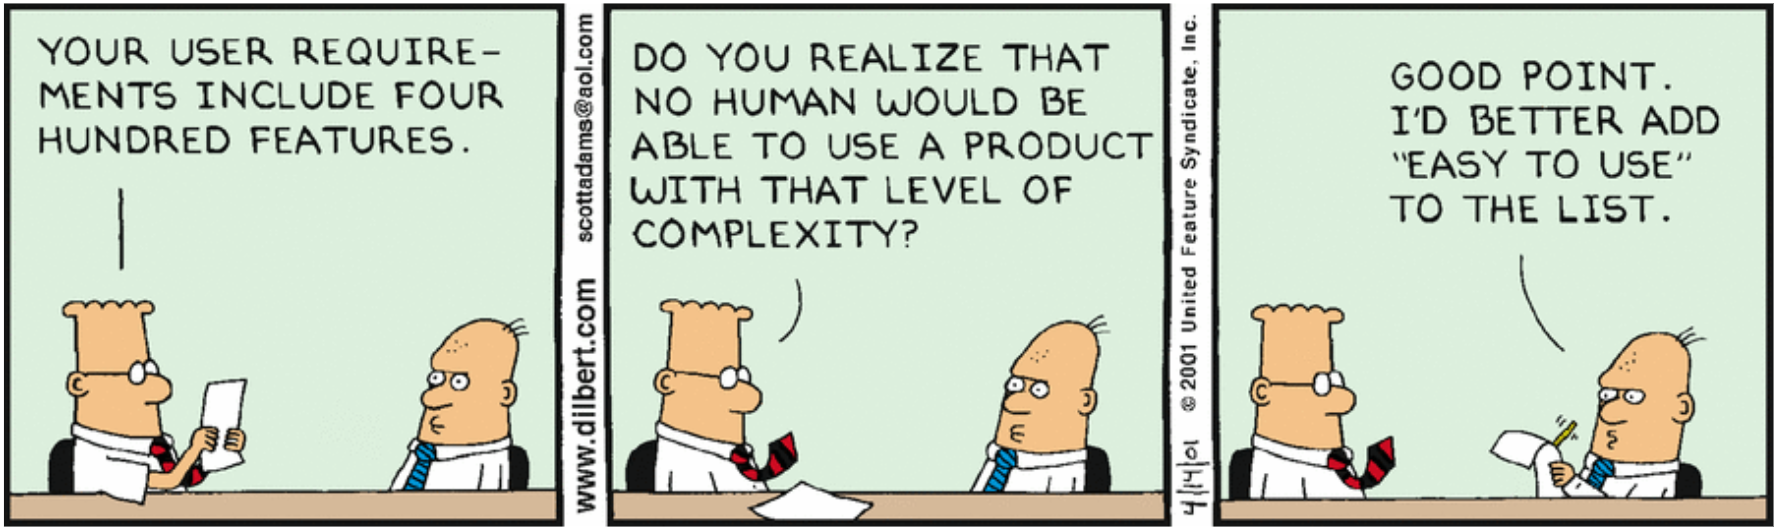
\includegraphics[width=0.95\textwidth]{dilbert.png}
        \end{center}
    \end{frame}

\end{document}
